\documentclass{ieeeaccess}

\usepackage{cite}
\usepackage{amsmath,amssymb,amsfonts}
\usepackage{booktabs}
\usepackage{tabularx}
\usepackage{multirow}
\usepackage{siunitx}
\usepackage{graphicx}
\usepackage{textcomp}
\usepackage{xcolor}
\usepackage{microtype}
\usepackage{hyperref}
\usepackage{float}
\usepackage{placeins}
\usepackage{dblfloatfix}
\usepackage{bm}

\makeatletter
\AtBeginDocument{\DeclareMathVersion{bold}
\SetSymbolFont{operators}{bold}{T1}{times}{b}{n}
\SetSymbolFont{NewLetters}{bold}{T1}{times}{b}{it}
\SetMathAlphabet{\mathrm}{bold}{T1}{times}{b}{n}
\SetMathAlphabet{\mathit}{bold}{T1}{times}{b}{it}
\SetMathAlphabet{\mathbf}{bold}{T1}{times}{b}{n}
\SetMathAlphabet{\mathtt}{bold}{OT1}{pcr}{b}{n}
\SetSymbolFont{symbols}{bold}{OMS}{cmsy}{b}{n}
\renewcommand\boldmath{\@nomath\boldmath\mathversion{bold}}}
\makeatother

\hypersetup{
  colorlinks=true,
  linkcolor=blue,
  citecolor=blue,
  urlcolor=blue
}

\graphicspath{{figures/}}

% Convenience macros
\newcommand{\cosa}{CoSA}
\newcommand{\Fonec}{$\mathrm{F1}_c$}
\newcommand{\Iouc}{$\mathrm{IoU}_c$}
\newcommand{\PrecC}{$\mathrm{Prec}_c$}
\newcommand{\RecC}{$\mathrm{Rec}_c$}

\begin{document}
\history{Date of publication xxxx 00, 0000, date of current version March 12, 2026.}
\doi{10.1109/ACCESS.2026.0000000}

\title{\cosa{}: Correlation-Guided Change Attention with Learnable Residual Gating for Remote Sensing Change Detection}

\author{\uppercase{Abdirashid Omar}\authorrefmark{1} and \uppercase{Jonghyuk Park}\authorrefmark{1}}
\address[1]{Department of Data Science, Graduate School of Kookmin University, Seoul, Republic of Korea}
\tfootnote{Code and materials: \href{https://github.com/rashiedomar/CoSA}{github.com/rashiedomar/CoSA}. Experiments use four datasets: LEVIR-CD, S2Looking, DSIFN, and CLCD.}
\markboth
{Omar and Park: \cosa{} for Remote Sensing Change Detection}
{Omar and Park: \cosa{} for Remote Sensing Change Detection}
\corresp{Corresponding author: Jonghyuk Park (e-mail: jonghyuk@kookmin.ac.kr).}

\begin{abstract}
Remote sensing change detection (CD) from bi-temporal imagery is critical for applications such as urban monitoring, disaster assessment, and environmental management, yet robust localization remains challenging under sparse changes, noisy labels, and appearance variations.
In this paper, we propose Context Sampling Attention (CoSA), a lightweight decoder-side refinement module that explicitly leverages bi-temporal feature correlation as a control signal for adaptive change-aware feature enhancement. This differs from conventional attention mechanisms that rely on implicit feature weighting without explicit temporal control. CoSA performs targeted refinement by selectively sampling correlation-relevant context, aggregating multi-scale information, and adaptively injecting it through learnable residual gating. This design enables effective discrimination between stable and ambiguous regions without relying on computationally expensive global attention.

Extensive experiments on four benchmark datasets (LEVIR-CD, S2Looking, DSIFN, and CLCD) demonstrate consistent improvements over strong baselines, achieving 1.5--2.6\% gains in changed-class F1 while introducing negligible parameter overhead. Ablation studies confirm that the synergy between correlation-guided sampling, multi-scale aggregation, and residual gating is essential for optimal performance.

These results indicate that CoSA establishes a practical and effective refinement paradigm for enhancing temporal discriminability in Siamese change detection frameworks.

\end{abstract}

\begin{keywords}
change detection, remote sensing, Siamese network, decoder refinement, attention, correlation, plug-in module
\end{keywords}

\titlepgskip=-21pt
\maketitle
\raggedbottom

\section{Introduction}\label{sec:introduction}
Remote sensing change detection (CD) from bi-temporal imagery plays a critical role in a wide range of applications, including urban monitoring, disaster response, and environmental management \cite{aisha2023,jungeun2025,seda2022,kyaw2024,r2024,j2026}. With the increasing availability of high-resolution satellite imagery, modern CD systems are required to distinguish meaningful semantic changes from nuisance variations caused by illumination shifts, seasonal differences, and geometric inconsistencies \cite{devansh2025,zainoolabadien2020,k2024,sai2026}. Despite significant progress in deep learning-based approaches, achieving robust and consistent localization across diverse scenarios remains a challenging problem.

Recent advances in CD have been driven by Siamese convolutional networks, attention-enhanced architectures, and transformer-based models, which improve feature representation and temporal interaction \cite{daudt2018fully,chen2020stanet,chen2022bit,bandara2022changeformer}. However, these methods often struggle to balance multi-scale localization, false-positive suppression, and computational efficiency, particularly under sparse changes, noisy labels, and ambiguous boundaries \cite{yan2024,shanshan2024,wei2024,devansh2025}. In many cases, global attention mechanisms introduce high computational cost without effectively resolving local ambiguity. These limitations highlight the need for a more targeted and efficient refinement strategy that can adaptively enhance change-relevant regions while preserving stable context. Section~\ref{sec:related_work} reviews these prior directions and clarifies the design gap addressed by \cosa{}.


\subsection{Proposed Contribution: Context Sampling Attention}
To address this limitation in explicit temporal control, we propose Context Sampling Attention (\cosa{}), a lightweight decoder-side refinement module that explicitly utilizes bi-temporal feature correlation as a control signal for change-aware feature enhancement. Unlike conventional attention mechanisms that implicitly learn feature relevance, \cosa{} performs targeted refinement by selectively sampling correlation-relevant context and adaptively integrating it into decoder features.

Specifically, \cosa{} consists of three coordinated components: (i) correlation-guided local context sampling, which focuses on informative neighboring regions; (ii) multi-scale context aggregation, which captures both fine-grained boundaries and broader semantic structures; and (iii) learnable residual gating, which controls the strength of contextual refinement. This design enables \cosa{} to emphasize ambiguous or potentially changed regions while preserving stable background context, leading to improved temporal discriminability with minimal computational overhead.

Importantly, \cosa{} is designed as a plug-in module that can be seamlessly integrated into existing Siamese encoder--decoder architectures without modifying the backbone. This allows consistent performance gains while maintaining architectural simplicity and efficiency. Figure~\ref{fig:intro_cosa_overview} illustrates this intuition by contrasting high-correlation stable context with low-correlation change-relevant regions in the refinement process.

\begin{figure}[t]
  \centering
  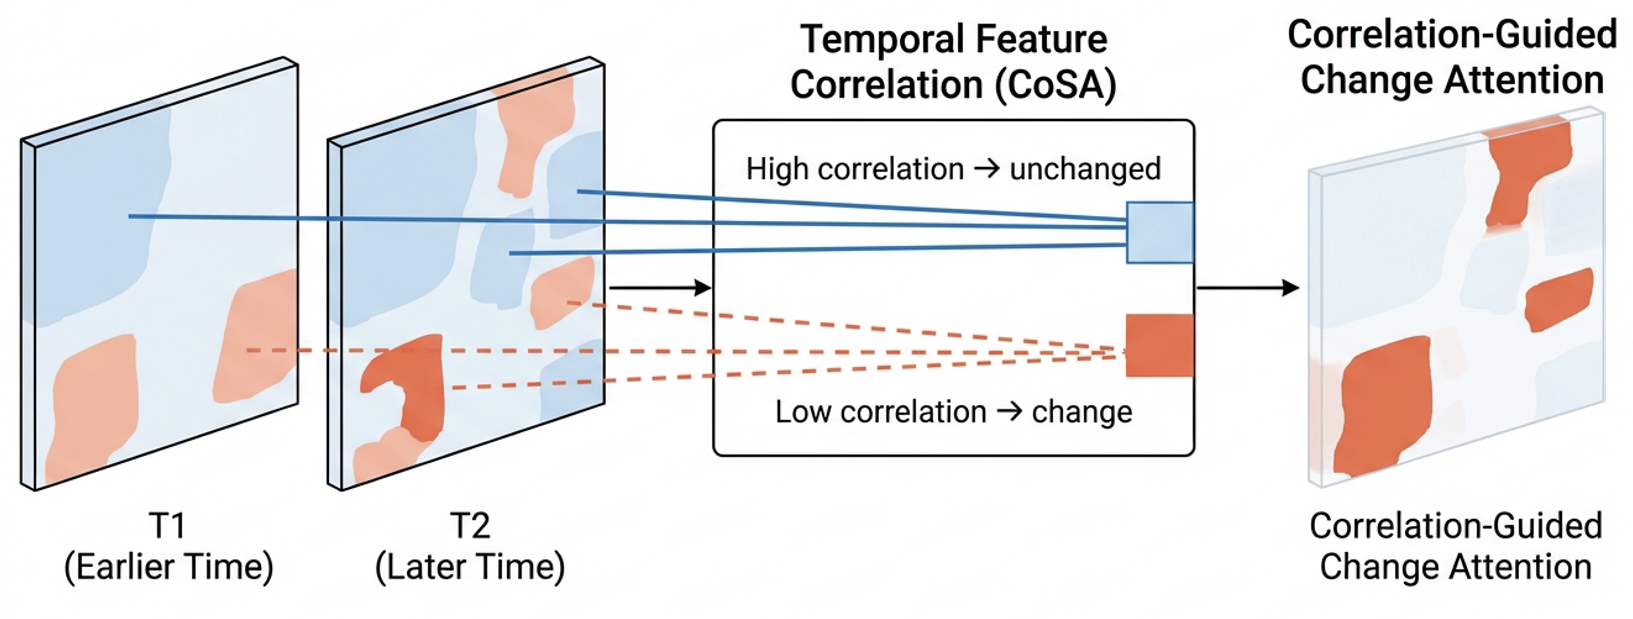
\includegraphics[width=\columnwidth]{example.png}
  \caption{Conceptual overview of \cosa{} in the introduction stage. Given bi-temporal features from \(T1\) and \(T2\), \cosa{} interprets high feature correlation as unchanged context and low correlation as potential change, then applies correlation-guided change attention for refined prediction.}
  \label{fig:intro_cosa_overview}
\end{figure}

\subsection{Evaluation Scope and Findings}
We evaluate \cosa{} on four benchmarks with complementary difficulty profiles: LEVIR-CD (clean building change), S2Looking (sparse off-nadir scenes), DSIFN (mixed urban-rural scenes), and CLCD (noisy agricultural boundaries). Across this suite, \cosa{} improves changed-class F1 by roughly 1.5--2.6 points with negligible parameter overhead. The improvement pattern is dataset-dependent: precision-oriented filtering on noisier or cluttered scenes, stronger recall recovery on ambiguous samples, and near-neutral behavior when the backbone already performs strong temporal fusion.

\subsection{Contributions}
\begin{itemize}
  \item We formulate CoSA as a plug-in decoder refinement module that treats bi-temporal correlation as an explicit control signal for where to refine, rather than relying solely on implicit feature reweighting.
  \item We integrate correlation-guided sampling, multi-scale aggregation, and learnable residual gating in one composite block; ablations show that peak performance requires this combination rather than any single component.
  \item On four benchmarks (LEVIR-CD, S2Looking, DSIFN, and CLCD), we report changed-class F1 gains of 1.5--2.6 points over strong baselines with negligible parameter overhead.
  \item On STANet and BIT, we observe large gains when temporal fusion is limited and near-neutral behavior when fusion is already strong.
\end{itemize}


\section{Related Work}\label{sec:related_work}
Remote sensing change detection has developed around four main deep-learning design families: Siamese CNN pipelines, attention-enhanced refinement networks, transformer-based temporal fusion models, and methods that make feature interaction more explicit through priors, flow, or matching. These lines of work address overlapping parts of the problem, but they differ sharply in temporal modeling, computational cost, and deployment practicality. This section positions \cosa{} within that landscape.

\subsection{CNN-Based Change Detection}
Foundational deep CD systems are largely Siamese CNN encoder--decoder models that process the two dates with shared weights and localize change through feature differencing or late fusion \cite{daudt2018fully,ronneberger2015unet,hongruixuan2019}. This design remains attractive because it is simple, efficient, and well aligned with pixel-wise CD supervision. Subsequent CNN variants improved decoder fusion and local representation quality through denser skip connections, deeper supervision, or lightweight multi-branch refinement, as seen in DSIFN \cite{zhang2020deeply}, SNUNet-CD \cite{fang2021snunetcd}, TinyCD \cite{codegoni2022tinycd}, LightCDNet \cite{10214556}, DASNet \cite{jie2020}, adaptive Siamese fusion \cite{yunzuo2025}, asymmetric semantic CD networks \cite{kunping2022}, and multitask Siamese designs \cite{xibing2025}.

These CNN-based methods establish strong practical baselines, but their temporal interaction is often dominated by fixed differencing or local convolutional fusion. As a result, long-range contextual reasoning, pseudo-change suppression, and precise boundary recovery remain difficult when changes are sparse, weak, or spatially ambiguous. The main limitation is therefore not feature extraction alone, but the lack of an explicit temporal control mechanism for decoder refinement. This limitation motivates \cosa{}, which strengthens temporal discrimination inside the decoder without abandoning the efficiency and simplicity of the Siamese CNN backbone.

\subsection{Attention-Based Methods}
Attention modules are a common extension to Siamese CNNs because they selectively reweight features that are likely to be useful for CD. STANet \cite{chen2020stanet} introduced spatial--temporal attention for remote sensing CD, while HANet \cite{10093022} and SemiSANet \cite{chengzhen2022} explored hierarchical and graph-attentive variants. Other works refine difference features with explicit attention branches, including AFDE-Net \cite{s2023}, ADDEDNet \cite{junheng2025}, and several multi-scale fusion architectures such as three-branch attention networks \cite{yan2024}, MDANet \cite{shanshan2024}, M2F2Net \cite{binhao2025}, wavelet-based aggregation \cite{jiangwei2024}, and lightweight multi-spectral attention models \cite{layth2025}.

These methods improve feature selection and often outperform plain CNN baselines, especially when multi-scale fusion is important. Their main limitation is that the attention mechanism is typically generic: it highlights informative channels or spatial regions, but it does not explicitly treat local bi-temporal correlation as a control variable for refinement. In addition, stacking multiple attention branches can erode the efficiency advantage of Siamese CNNs without fully resolving CD-specific issues such as pseudo-change suppression and stable precision/recall calibration. Accordingly, \cosa{} uses correlation-guided sampling to make temporal interaction explicit while keeping the refinement lightweight and locally focused.

\subsection{Transformer-Based Approaches}
Transformer-based CD models push temporal interaction further by using self-attention to capture long-range dependencies across the bi-temporal pair. Representative examples include BIT \cite{chen2022bit}, ChangeFormer \cite{bandara2022changeformer}, transformer-based Siamese CD \cite{w2022}, STransUNet \cite{jianghua2022}, multitask CNN--Transformer semantic CD \cite{wei2024}, and STeInFormer \cite{xiaowen2024}. More recent work has explored stronger pretraining and larger representation models, including bitemporal foundation-model integration \cite{chen2023time}, foundation-model-based remote sensing CD \cite{10438490}, and new large-scale evaluation settings such as JL1-CD \cite{liu2025jl1}. Recent reviews also show that transformer-style global fusion is now a major axis of CD research \cite{devansh2025,kamalakar2025}.

The trade-off is practical. Global attention improves contextual modeling, but it also increases memory and computational cost as image resolution grows, and many transformer solutions require backbone-level redesign rather than local refinement. Strong temporal fusion may also reduce the marginal value of later decoder enhancement, which is consistent with our near-neutral BIT result. The main limitation here is that stronger temporal modeling is often purchased through higher complexity and reduced plug-in compatibility. This limitation motivates \cosa{}, which targets adaptive temporal refinement at the decoder level without incurring the full cost of global all-pairs interaction.

\subsection{Correlation-Based and Feature Interaction Methods}
A smaller but important line of work tries to move beyond plain differencing by making cross-temporal interaction more explicit. Changer argues that feature interaction is central to CD and introduces dedicated interaction modeling \cite{fang2022changer}. Change Guiding Network injects a learned change prior to steer prediction \cite{10234560}, while SFSCDNet uses semantic flow to encode structured temporal correspondence \cite{k2024}. Related formulations also widen the supervision or interaction setting, for example by reframing object change detection with single-temporal supervision \cite{zheng2021change} or by integrating richer bi-temporal features through large pre-trained models \cite{chen2023time}.

These methods are closer to \cosa{} in spirit because they recognize that temporal correspondence should be modeled more deliberately. However, they generally treat interaction as another representation-learning block, change prior, or global fusion stage. They do not use local correlation as an explicit decoder-level control signal that decides where refinement should be strengthened or suppressed. They also rarely combine explicit temporal interaction with both multi-scale context aggregation and learnable residual calibration in one lightweight plug-in module. \cosa{} targets this gap by turning local correlation into an explicit decoder-side refinement signal and coupling it with multi-scale fusion and learnable residual control in a single plug-in design.

\subsection{Positioning \cosa{}}
\cosa{} is positioned between heavy backbone replacement and generic add-on attention. Relative to CNN baselines \cite{daudt2018fully,hongruixuan2019}, it injects stronger temporal discrimination without changing the encoder or prediction head. Relative to attention-based refinements \cite{chen2020stanet,10093022,yan2024}, it uses bi-temporal correlation explicitly rather than only reweighting features implicitly. Relative to transformer-style models \cite{chen2022bit,bandara2022changeformer,wei2024}, it keeps computation local and preserves plug-in compatibility. Relative to interaction- or prior-based designs \cite{fang2022changer,10234560,k2024}, it couples three coordinated mechanisms in the decoder: correlation-guided sampling, multi-scale fusion, and learnable residual gating.

That combination is the main distinction of \cosa{}. The module is designed for targeted decoder refinement rather than wholesale architectural replacement, and the ablation later in the paper shows that its gains do not come from any one component in isolation. Recent hybrid systems for specialized CD settings, such as SiamMask-ICDNet for island-building monitoring \cite{lebao2025}, further illustrate a broader trend: many gains come from scenario-specific redesign rather than from a general refinement block. \cosa{} instead targets the unresolved design gap of a lightweight mechanism that uses local temporal correlation as an explicit control signal while remaining deployable across heterogeneous Siamese backbones.


\section{Method}\label{sec:method}
We present Context Sampling Attention (\cosa{}) as a lightweight decoder-side refinement module for Siamese change detection pipelines. The method is designed to be interpretable, computationally efficient, and plug-in compatible with existing encoder--decoder systems. Its central novelty is that local bi-temporal correlation is used as an explicit decoder-side control signal for refinement, rather than being left as an implicit byproduct of generic attention or backbone fusion.

\subsection{Overview and Architecture}
Given a bi-temporal pair $(I_1, I_2)$, a Siamese encoder extracts multi-scale features and a differencing operator produces decoder-level change-aware tensors, following common FC-Siam-style practice \cite{daudt2018fully,hongruixuan2019,ronneberger2015unet}. \cosa{} is inserted at selected decoder stages (typically 1/8 and 1/16 resolution) to refine these difference features without changing the encoder or prediction head.

\noindent\textbf{Design principle.} Rather than replacing the backbone with global self-attention, \cosa{} performs localized decoder refinement where change/no-change ambiguity is resolved. This keeps architectural disruption low while improving temporal discriminability. The proposed architecture is depicted in Figure~\ref{fig:arch}, which shows where \cosa{} is inserted in the decoder and how correlation-guided sampling, multi-scale fusion, and residual-gated refinement are applied before downstream decoding.

\begin{figure*}[!t]
  \centering
  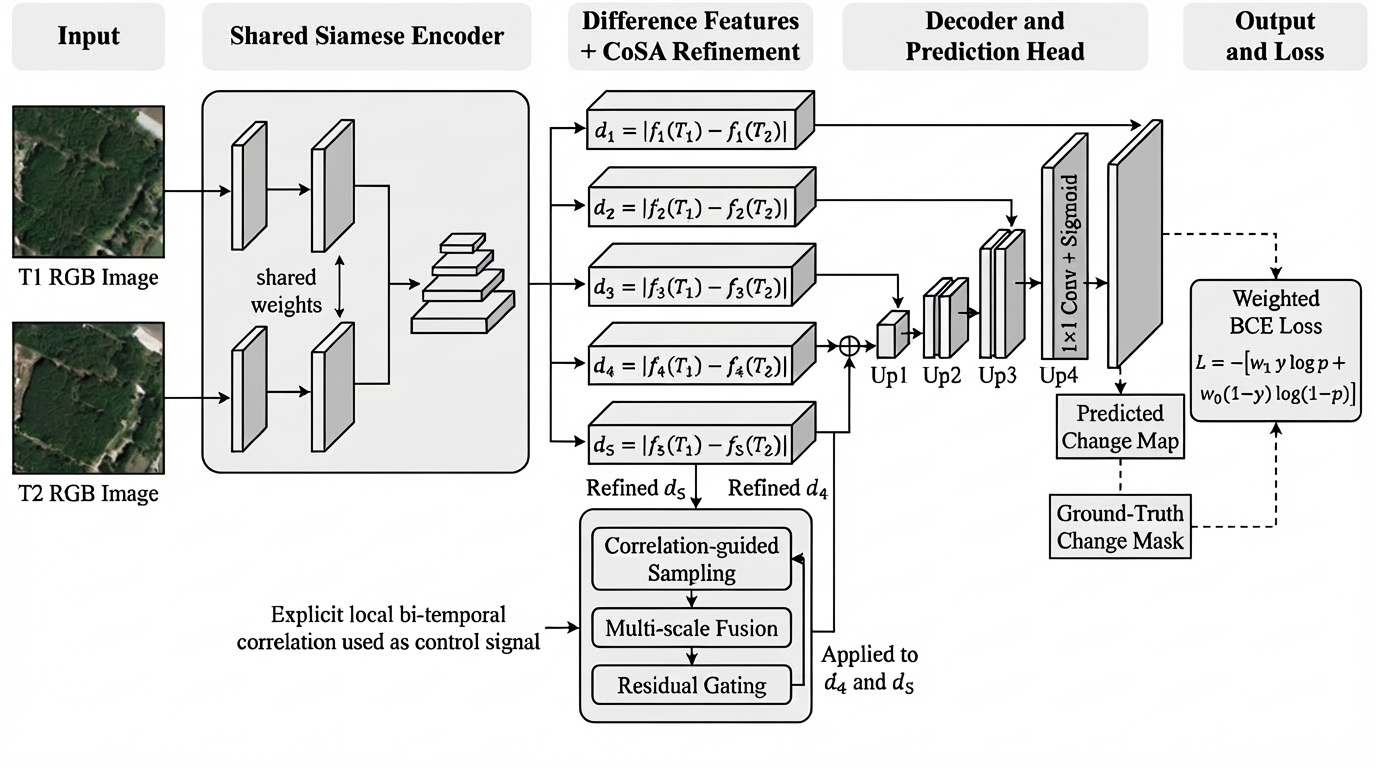
\includegraphics[width=\textwidth]{model_architecture.png}
  \caption{Full FC-Siam-style pipeline with \cosa{} inserted at selected decoder stages. The figure shows the bi-temporal inputs, shared Siamese encoder, multi-scale difference features, \cosa{} refinement applied to deep difference features, progressive decoding, final change-map prediction, and the weighted BCE loss used during training.}
  \label{fig:arch}
\end{figure*}

\subsection{Correlation-Based Context Sampling}
\noindent\textbf{Intuition.} Temporal correlation provides a practical signal for refinement control. High local correlation generally indicates stable unchanged context, while low correlation often appears near changed or ambiguous regions.

Unlike standard attention mechanisms that compute soft weights over all neighbors, \cosa{} first filters the neighborhood through correlation relevance and then aggregates only the selected context. This makes the refinement decision explicit, sparse, and directly tied to temporal agreement rather than generic feature weighting.

Let $F_{\text{diff}} \in \mathbb{R}^{H \times W \times C}$ be a decoder difference feature map. For each position $(x,y)$ and neighbor $p \in \mathcal{N}(x,y)$, we compute:
\begin{equation}
\mathrm{Corr}(x,y,p) = F_{\text{diff}}(x,y)\cdot F_{\text{diff}}(p),
\end{equation}
where $\cdot$ denotes channel-wise inner product.

We keep only correlation-relevant neighbors:
\begin{equation}
\mathcal{N}_{\text{corr}}(x,y)=\left\{p\in\mathcal{N}(x,y): \mathrm{Corr}(x,y,p)>\tau \right\},
\end{equation}
and aggregate selected context by a lightweight operator:
\begin{equation}
\mathrm{Ctx}(x,y)=\mathrm{Agg}\!\left(\left\{F_{\text{diff}}(p): p \in \mathcal{N}_{\text{corr}}(x,y)\right\}\right).
\end{equation}
Here, $\tau$ is a sampling threshold (fixed or learnable), and $\mathrm{Agg}(\cdot)$ is mean/max or a lightweight learned combiner.

Compared with dense global attention, this local sampling reduces complexity from global pairwise interaction to neighborhood interaction, with practical cost $O(HWk^2C)$ for a $k \times k$ window.

\subsection{Multi-Scale Context Integration}
Change cues span multiple scales: fine boundaries require high-resolution detail, while large-area changes require coarser semantic context. We therefore fuse correlation-guided context across decoder scales:
\begin{equation}
\begin{aligned}
\mathrm{Ctx}_{\text{multi}}(x,y)=\mathrm{Concat}\big(&\mathrm{Ctx}^{(1)}(x,y),\ldots,\\
&\mathrm{Ctx}^{(N)}(x,y)\big),
\end{aligned}
\end{equation}
where coarser contexts are upsampled to the target scale before concatenation.

This design preserves both local boundary structure and broader scene consistency, consistent with multi-scale principles used in modern CD decoders \cite{yan2024,shanshan2024,binhao2025}. In \cosa{}, multi-scale integration is particularly important because correlation-guided sampling may capture different change patterns at different spatial resolutions. When needed, a $1\times1$ projection compresses concatenated channels before gating to control parameter growth.

\subsection{Learnable Residual Gating}
Refined context is injected through residual gating:
\begin{equation}
F_{\text{refined}} = F_{\text{base}} + \lambda \odot \mathrm{Ctx}_{\text{multi}},
\end{equation}
where $\lambda$ is a learnable gate (scalar, channel-wise, or element-wise) and $\odot$ is element-wise multiplication.

While residual gating itself is not new, its role in \cosa{} is different from generic residual scaling modules that simply rescale fused decoder features after aggregation. In \cosa{}, the gate modulates only correlation-sampled multi-scale context, so the network decides how much temporally supported evidence should be injected into the decoder at each location and scale. This makes the gate part of the explicit temporal-control mechanism rather than a generic stabilization trick. If the sampled context is unhelpful, \cosa{} suppresses refinement through small $\lambda$; if the context is informative, it amplifies refinement. Residual gating therefore decouples \emph{what to sample} from \emph{how strongly to apply it}, giving \cosa{} adaptive decoder-side control with far lower overhead than heavy global interaction modules \cite{w2022,wei2024,xiaowen2024}.

\subsection{Training Objective}
\cosa{} does not introduce an auxiliary supervision branch; it is trained with the same pixel-wise changed/unchanged objective used by the underlying CD model. Let $Y \in \{0,1\}^{H \times W}$ denote the ground-truth change mask and $\hat{P} \in [0,1]^{H \times W}$ the predicted changed-class probability map. We optimize a weighted binary cross-entropy loss:
\begin{equation}
\begin{aligned}
\mathcal{L}_{\text{wBCE}} = - \sum_{x,y} \big[& w_1 Y_{x,y}\log \hat{P}_{x,y} \\
&+ w_0(1-Y_{x,y})\log(1-\hat{P}_{x,y})\big],
\end{aligned}
\end{equation}
where $w_1$ and $w_0$ balance the changed and unchanged classes, respectively. In our controlled experiments, we use the same unchanged:changed weighting ratio of $1:3$ for both the baseline and \cosa{}, so performance differences reflect decoder refinement rather than a modified loss design. The full optimization recipe is given in the experimental protocol section.

\subsection{Module Workflow and Integration}
At each selected decoder stage, \cosa{} executes:
\begin{enumerate}
  \item compute difference features from bi-temporal decoder activations;
  \item perform correlation-guided context sampling (possibly at multiple scales);
  \item fuse sampled context and apply residual gating;
  \item pass refined features to subsequent decoder operations.
\end{enumerate}

\noindent\textbf{Integration scope.} \cosa{} is plug-and-play: encoder backbone, differencing strategy, and prediction head remain unchanged. In our setup, practical defaults are a $3\times3$ neighborhood, two decoder scales (1/8 and 1/16), and near-zero gate initialization for stable warm-up.

\subsection{Method-Level Novelty Summary}
The novelty of \cosa{} lies in its explicit use of local bi-temporal correlation as a control signal, combined with a coordinated refinement design that integrates correlation-guided sampling, multi-scale fusion, and adaptive residual gating. This combination enables a form of targeted refinement that is not achievable by conventional attention or single-component designs.


\section{Experiments}\label{sec:experiments}
This section defines the datasets, metrics, and evaluation protocol used to assess \cosa{} under controlled and transfer settings. Table~\ref{tab:datasets} summarizes the four benchmark datasets used throughout the section (scale, splits, and resolution).

\begin{table*}[t]
  \centering
  \caption{Dataset statistics and download links.}
  \label{tab:datasets}
  \setlength{\tabcolsep}{7pt}
  \renewcommand{\arraystretch}{1.08}
  \small
  \begin{tabular}{l c c c c c c}
    \toprule
    Dataset & Task & Image Pairs & Image Size & Change Instances & Change Pixels & Download \\
    \midrule
    LEVIR-CD & binary & 637 & 1024$\times$1024 & 31K & 30M & \href{https://github.com/justchenhao/LEVIR}{URL} \\
    S2Looking & binary & 5,000 & 1024$\times$1024 & 66K & 69M & \href{https://github.com/S2Looking/Dataset}{URL} \\
    DSIFN & binary & 394 & 512$\times$512 & -- & -- & \href{https://geozcx.github.io/A-deeply-supervised-image-fusion-network-for-change-detection-in-remote-sensing-images/}{URL} \\
    CLCD & binary & 560 & 512$\times$512 & -- & -- & \href{https://github.com/liumency/CropLand-CD}{URL} \\
    \bottomrule
  \end{tabular}
\end{table*}


\subsection{Datasets and Evaluation Metrics}
We evaluate on four benchmarks with complementary difficulty profiles: LEVIR-CD \cite{chen2020stanet}, S2Looking \cite{s2looking_dataset}, DSIFN \cite{dsifn_dataset}, and CLCD \cite{clcd_dataset}. This selection intentionally spans clean urban building change (LEVIR-CD), sparse off-nadir scenes (S2Looking), mixed urban-rural conditions (DSIFN), and noisy agricultural boundaries (CLCD), so claims are not tied to one favorable benchmark. The statistics and sources in Table~\ref{tab:datasets} make clear that the four benchmarks differ substantially in annotation richness and scene structure.

Figure~\ref{fig:training_dynamics} shows training loss for the controlled FC-Siam baseline and FC-Siam+\cosa{} runs on each of the four datasets under the shared protocol.

\begin{figure*}[!t]
  \centering
  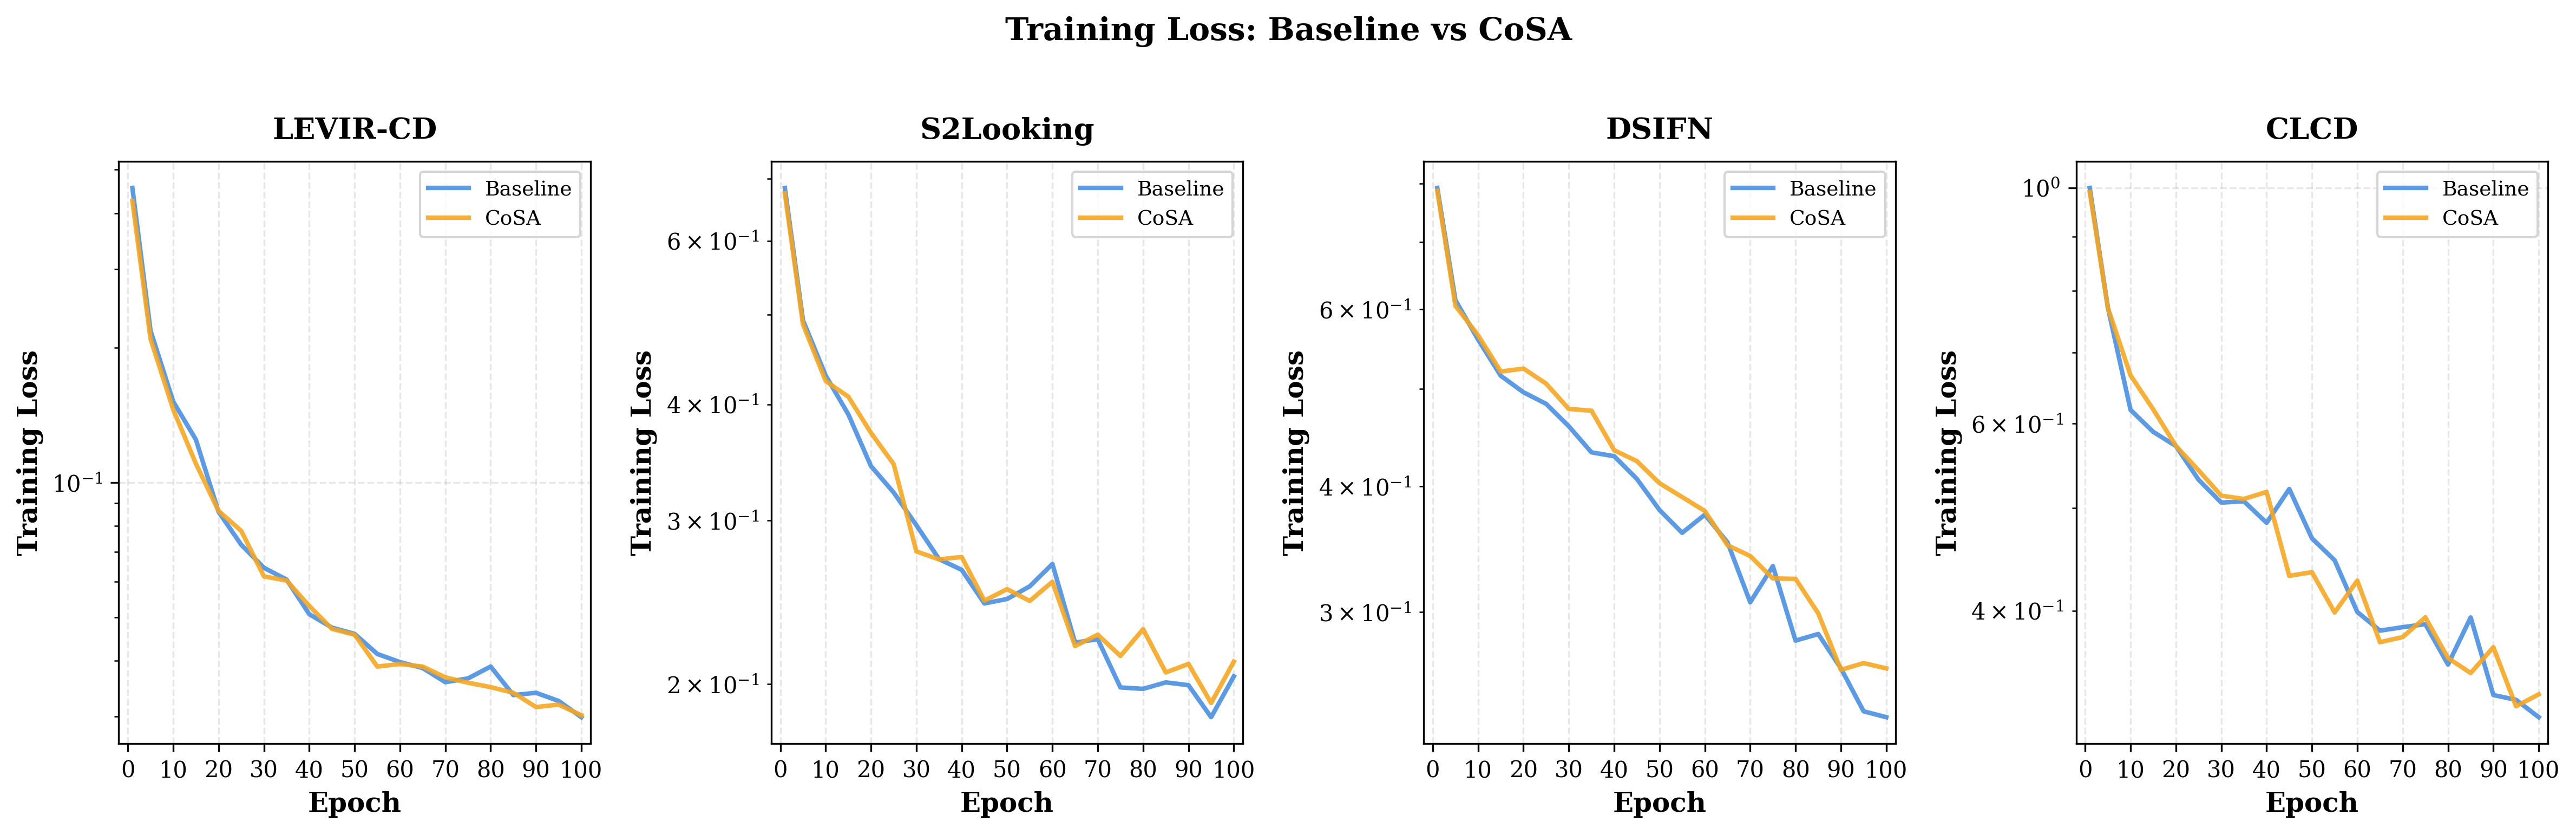
\includegraphics[width=\textwidth]{training_loss_all_datasets.png}
  \caption{Training loss for the FC-Siam baseline and FC-Siam+\cosa{} across LEVIR-CD, S2Looking, DSIFN, and CLCD.}
  \label{fig:training_dynamics}
\end{figure*}

These four datasets are sufficient for evaluating generality because, taken together, they cover the main axes on which remote sensing CD methods typically fail: clean versus noisy annotation, dense versus sparse change, stable versus off-nadir acquisition, and relatively sharp versus ambiguous boundaries. LEVIR-CD provides a relatively clean, high-quality setting with limited headroom; S2Looking stresses sparse and ambiguous changes under viewpoint variation; DSIFN represents intermediate real-world complexity; and CLCD stresses robustness to noisy boundaries and label uncertainty. A method that improves consistently across all four is therefore less likely to be benefiting from dataset cherry-picking and more likely to be addressing a transferable refinement problem.

Following standard CD reporting, we use changed-class precision, recall, F1, and IoU (\PrecC{}, \RecC{}, \Fonec{}, \Iouc{}) \cite{devansh2025,kamalakar2025}:
\begin{equation}
\mathrm{Prec}_c=\frac{TP}{TP+FP}, \quad \mathrm{Rec}_c=\frac{TP}{TP+FN},
\end{equation}
\begin{equation}
\mathrm{F1}_c=\frac{2\cdot \mathrm{Prec}_c\cdot \mathrm{Rec}_c}{\mathrm{Prec}_c+\mathrm{Rec}_c}, \quad \mathrm{IoU}_c=\frac{TP}{TP+FP+FN}.
\end{equation}
These metrics capture false-alarm suppression (precision), missed-change recovery (recall), overall discrimination (F1), and spatial overlap quality (IoU).

\subsection{Experimental Settings and Protocol}
To isolate architectural effects, baseline and \cosa{} share identical settings: a Siamese U-Net-style decoder \cite{ronneberger2015unet} with a ResNet-18 backbone \cite{he2016resnet}, absolute differencing, weighted cross-entropy (unchanged:changed = 1:3), Adam ($\beta_1=0.9$, $\beta_2=0.999$), initial learning rate $10^{-4}$, and a ReduceLROnPlateau scheduler that monitors validation \Fonec{} and halves the learning rate when the score fails to improve for 10 epochs. Training uses batch size 8 for up to 100 epochs with early stopping (patience 15) and seed 42. We use standard augmentation (flip, rotation, and light color jitter), select checkpoints by validation \Fonec{}, and report test metrics at a 0.5 sigmoid threshold. For LEVIR-CD, the split is 445 training images, 64 validation images, and 128 test images. For S2Looking, DSIFN, and CLCD, we use fixed train/validation/test splits documented in the released configs to ensure reproducibility. Standalone STANet and BIT experiments are run under their native/custom pipelines to evaluate plug-in compatibility under model-preferred recipes; these are reported in Subsection~\ref{sec:hero_models}.

\subsection{Baseline vs \cosa{}}
Table~\ref{tab:fcsiam_vs_cosa} reports controlled test-set results for the FC-Siam baseline and FC-Siam+\cosa{} across all four datasets.

\begin{table*}[t]
  \centering
  \caption{Performance comparison between the FC-Siam baseline and \cosa{} on four change detection benchmarks.}
  \label{tab:fcsiam_vs_cosa}
  \setlength{\tabcolsep}{6pt}
  \renewcommand{\arraystretch}{1.08}
  \small
  \begin{tabular*}{\textwidth}{@{\extracolsep{\fill}} l l r r r r r r}
    \toprule
    Dataset & Method & \Fonec{} (\%) & \Iouc{} (\%) & \PrecC{} (\%) & \RecC{} (\%) & $\Delta \mathrm{F1}_c$ & $\Delta \mathrm{IoU}_c$ \\
    \midrule
    \textbf{LEVIR-CD} & FC-Siam baseline & 87.70 & 78.09 & 90.23 & 85.31 & --- & --- \\
    & \cosa{} & \textbf{89.45} & \textbf{80.91} & \textbf{90.39} & \textbf{88.52} & \textbf{+1.75} & \textbf{+2.82} \\
    \midrule
    \textbf{DSIFN} & FC-Siam baseline & 74.85 & 59.81 & \textbf{82.05} & 68.81 & --- & --- \\
    & \cosa{} & \textbf{76.52} & \textbf{61.98} & 68.61 & \textbf{86.50} & \textbf{+1.67} & \textbf{+2.17} \\
    \midrule
    \textbf{CLCD} & FC-Siam baseline & 46.94 & 30.67 & 34.16 & \textbf{75.04} & --- & --- \\
    & \cosa{} & \textbf{49.53} & \textbf{32.91} & \textbf{41.97} & 60.40 & \textbf{+2.59} & \textbf{+2.24} \\
    \midrule
    \textbf{S2Looking} & FC-Siam baseline & 38.00 & 23.46 & 24.93 & 79.82 & --- & --- \\
    & \cosa{} & \textbf{40.44} & \textbf{25.34} & \textbf{26.99} & \textbf{80.58} & \textbf{+2.44} & \textbf{+1.88} \\
    \bottomrule
  \end{tabular*}
\end{table*}


\cosa{} improves \Fonec{} and \Iouc{} on all four datasets, with \Fonec{} gains from +1.67 to +2.59 and \Iouc{} gains from +1.88 to +2.82. Although the numerical gains may appear modest, they are consistent across all datasets and achieved with negligible parameter overhead. The largest gains appear on S2Looking and CLCD, where sparse changes and noisy boundaries make selective context aggregation more valuable. The gains are not uniform: on LEVIR-CD, \cosa{} preserves precision and improves recall (+3.21 points), indicating stronger missed-change recovery without clear false-alarm inflation; on CLCD, precision rises strongly (+7.81) while recall decreases, indicating conservative false-positive filtering in noisy conditions; DSIFN shows a recall-oriented shift with reduced precision, while S2Looking improves both precision and recall modestly. This behavior reflects the adaptive nature of \cosa{}, which adjusts refinement based on dataset characteristics. The training-loss curves in Figure~\ref{fig:training_dynamics} are consistent with this pattern: \cosa{} typically converges to lower loss and stabilizes earlier across the four datasets. This dataset-dependent behavior motivates the deeper error analysis in Section~\ref{sec:analysis}.

Figure~\ref{fig:baseline_cosa_qual_all_datasets} shows representative predictions on one strong-gain test sample per dataset (same protocol as Table~\ref{tab:fcsiam_vs_cosa}): baseline overlays (TP green, FP red), \cosa{} overlays, and \cosa{} gain (blue) with remaining FP (red).

\begin{figure*}[!t]
  \centering
  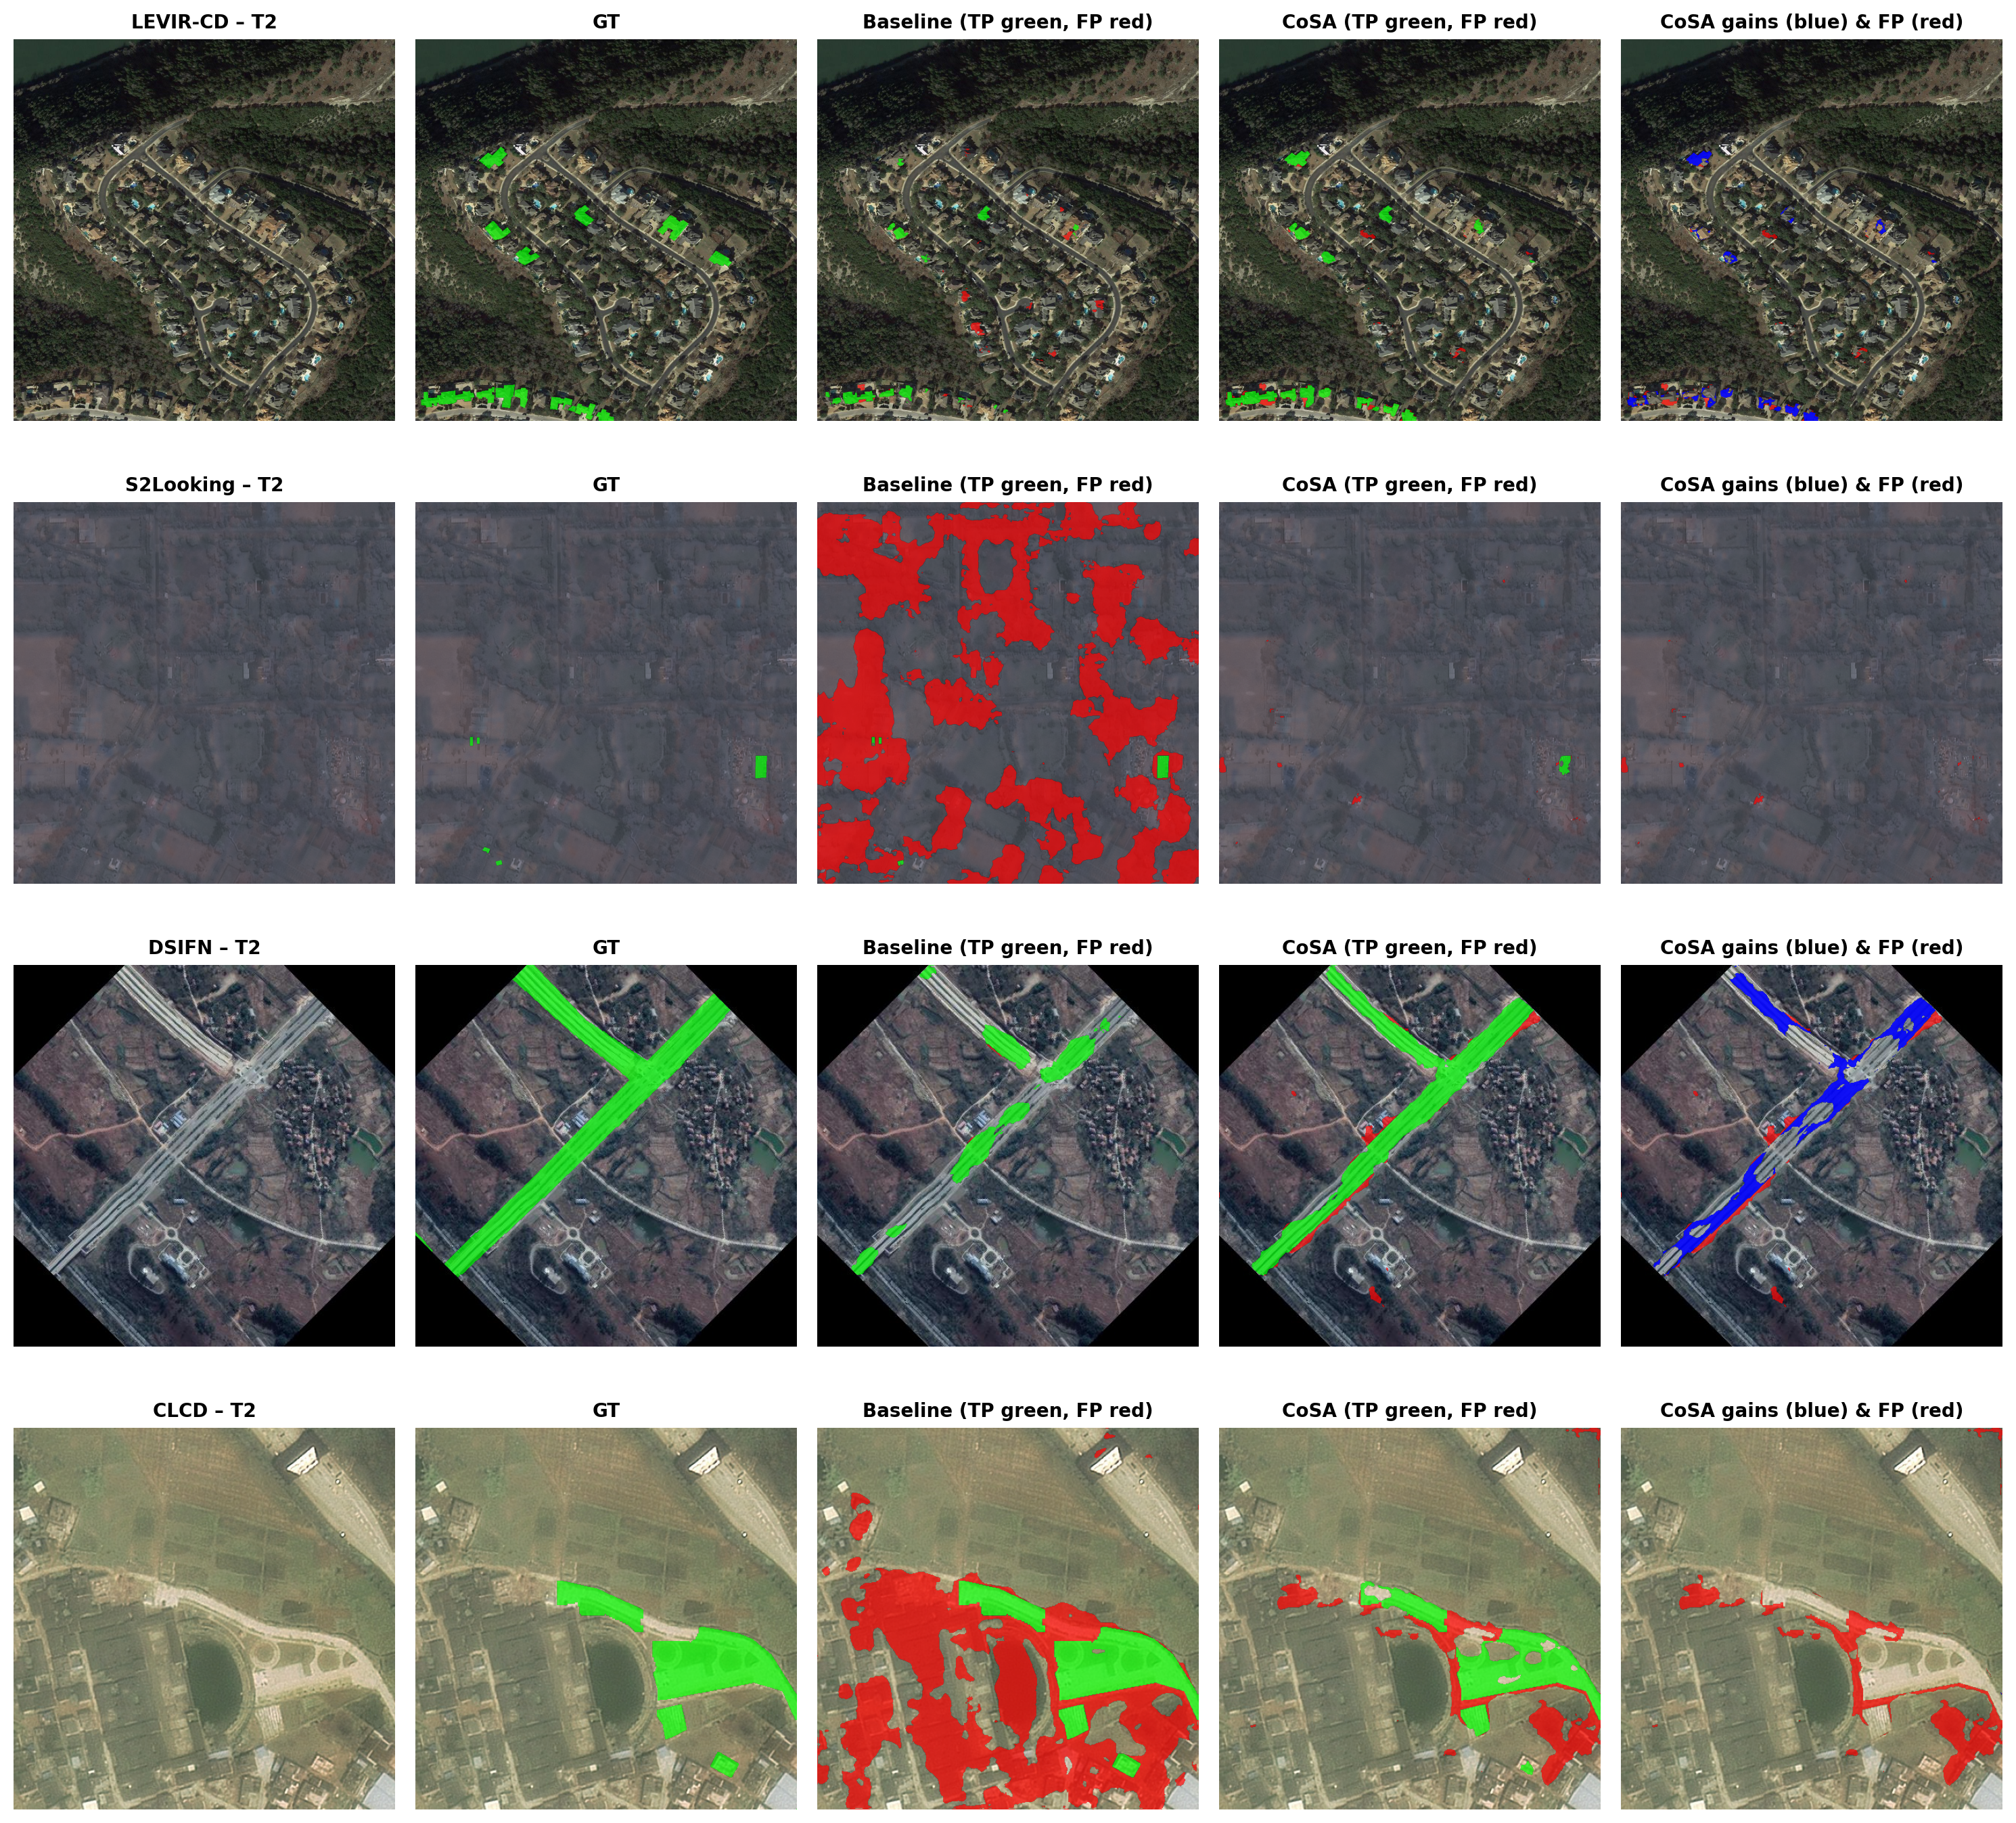
\includegraphics[width=\textwidth]{baseline_cosa_qual_all_datasets.png}
  \caption{Qualitative baseline-vs-\cosa{} comparison across LEVIR-CD, S2Looking, DSIFN, and CLCD. Columns (left to right): T2 image, ground truth, baseline overlay (TP green, FP red), \cosa{} overlay (TP green, FP red), and \cosa{} gains (blue) with remaining FP (red).}
  \label{fig:baseline_cosa_qual_all_datasets}
\end{figure*}

The visual trends align with Table~\ref{tab:fcsiam_vs_cosa}: reduced false positives in sparse/noisy scenes and improved coverage of weak true changes in ambiguous regions.

We isolate mechanism-level evidence in Subsection~\ref{sec:ablation}, test cross-backbone transferability in Subsection~\ref{sec:hero_models}, and analyze FP/FN transitions with patch-level consistency in Section~\ref{sec:analysis}.

\subsection{Reproducibility}
We fix training and data-loading seeds (including seed 42 for the controlled FC-Siam runs), save the best checkpoint by validation \Fonec{}, and cache per-sample predictions used for analysis tables. Paper tables and figures are generated from those logged artifacts. Full datasets and large checkpoints are omitted from the public repository for size, but released code includes configuration files, split definitions, training scripts, and evaluation commands sufficient to reproduce the reported metrics on the same public benchmarks.

\subsection{Ablation Study}\label{sec:ablation}
We conduct an ablation study over multiple variants on the same FC-Siam-diff-style backbone: baseline, attention-only, \cosa{} with multi-scale only, \cosa{} with gate only, \cosa{} with single-scale and fixed gate, alignment-first, and the full \cosa{} configuration with multi-scale refinement and learnable gating.

Table~\ref{tab:ablation} lists quantitative results for each variant on LEVIR-CD. Figure~\ref{fig:ablation_qualitative} complements Table~\ref{tab:ablation} with qualitative error maps (false positives and false negatives) for the same setting.

% Table 2: CoSA ablation study (variants / components)
% Source: ablation/ablation_study/ablation_summary.json
\begin{table*}[t]
  \centering
  \caption{Ablation study on LEVIR-CD (changed class).}
  \label{tab:ablation}
  \setlength{\tabcolsep}{6pt}
  \renewcommand{\arraystretch}{1.05}
  \small
  \begin{tabularx}{\textwidth}{X r r r r}
    \toprule
    Variant & \PrecC{} & \RecC{} & \Fonec{} & \Iouc{} \\
    \midrule
    Baseline & 90.23 & 85.31 & 87.70 & 78.09 \\
    Attention-only & 90.27 & 85.61 & 87.88 & 78.38 \\
    \cosa{} with multi-scale only & 91.35 & 83.68 & 87.35 & 77.54 \\
    \cosa{} with gate only & 93.33 & 82.67 & 87.68 & 78.06 \\
    \cosa{} with single-scale and fixed gate & \textbf{93.88} & 83.22 & 88.23 & 78.94 \\
    Alignment-first & 92.00 & 85.62 & 88.70 & 79.69 \\
    Full \cosa{} (multi-scale + learnable gate; ours) & 90.39 & \textbf{88.52} & \textbf{89.45} & \textbf{80.91} \\
    \bottomrule
  \end{tabularx}
\end{table*}


\begin{figure}[!t]
  \centering
  \includegraphics[width=\columnwidth]{ablation_qualitative_alt3_errors_only_v2.png}
  \caption{Qualitative ablation comparison (errors only): highlighted regions emphasize false positives and false negatives across variants.}
  \label{fig:ablation_qualitative}
\end{figure}

``Multi-scale'' inserts \cosa{} at two resolutions (1/8 and 1/16). ``Learnable gate'' uses a trainable residual scale $\lambda$ (Section~\ref{sec:method}) initialized near zero; fixed-scale uses a constant residual factor. ``Gate only'' disables multi-scale placement and keeps only residual gating at the bottleneck. ``Alignment-first'' estimates local displacement and warps features before differencing. The full \cosa{} configuration (multi-scale + learnable residual scale) gives the best F1/IoU balance among tested variants. Relative to baseline, \cosa{} improves recall (+3.21 points) with near-stable precision (+0.16 points), yielding +1.75 \Fonec{} and +2.82 \Iouc{}. The single-scale fixed variant improves precision but reduces recall, indicating that correlation refinement without adaptive residual control can become overly conservative. The alignment-first variant improves over baseline but remains below full \cosa{}, suggesting that adaptive correlation-guided refinement is more effective than geometric pre-alignment alone in this setup \cite{shanshan2024,yan2024}. Table~\ref{tab:ablation} therefore provides the experimental evidence for the method-level claim: multi-scale sampling alone or gating alone is insufficient for peak performance, and the full gain appears only when correlation-guided sampling, multi-scale fusion, and adaptive residual control are used together. This combination enables a form of targeted refinement that is not achievable by conventional attention or single-component designs. Figure~\ref{fig:ablation_qualitative} illustrates where partial variants fail: the full module suppresses spurious detections while recovering missing change regions more consistently than partial variants.

\subsection{Standalone Hero Models}\label{sec:hero_models}
We report standalone ``hero'' experiments for STANet \cite{chen2020stanet} and BIT \cite{chen2022bit} under their native/custom pipelines. The goal is to test transferability of \cosa{} when inserted into strong non-baseline backbones.
Table~\ref{tab:hero_models} reports the changed-class results for these two backbones and shows that \cosa{} delivers a large gain on STANet but only a marginal change on BIT.

\begin{table*}[t]
  \centering
  \caption{Standalone hero models under their native pipelines (changed class).}
  \label{tab:hero_models}
  \setlength{\tabcolsep}{7pt}
  \renewcommand{\arraystretch}{1.05}
  \small
  \begin{tabular*}{\textwidth}{@{\extracolsep{\fill}} l l r r r r}
    \toprule
    Model & Variant & \PrecC{} & \RecC{} & \Fonec{} & \Iouc{} \\
    \midrule
    STANet & Baseline & 70.31 & \textbf{94.71} & 80.71 & 67.66 \\
    STANet & + \cosa{} & \textbf{87.11} & 85.19 & \textbf{86.14} & \textbf{75.66} \\
    BIT & Baseline & 91.37 & \textbf{91.08} & 91.22 & 83.87 \\
    BIT & + \cosa{} & \textbf{92.38} & 90.17 & \textbf{91.26} & \textbf{83.93} \\
    \bottomrule
  \end{tabular*}
\end{table*}


The two hero models exhibit clearly different responses. On STANet, \cosa{} provides a large gain (\Fonec{}: 80.71 \textrightarrow 86.14; \Iouc{}: 67.66 \textrightarrow 75.66) with a strong precision increase, indicating effective suppression of over-detection. On BIT, the effect is near-neutral (\Fonec{}: 91.22 \textrightarrow 91.26), consistent with partial redundancy between explicit correlation gating and BIT's transformer-based temporal interaction. Standalone evidence therefore matches the broader pattern in this paper: \cosa{} is most beneficial when it complements, rather than duplicates, the temporal interaction already encoded by the backbone \cite{w2022,wei2024}.


\section{Analysis}\label{sec:analysis}
This section moves beyond aggregate scores to analyze \emph{how} \cosa{} changes errors, \emph{where} gains occur at sample level, and \emph{why} behavior differs across datasets and backbones.

\subsection{Error Correction Mechanics: FP/FN Transitions}
To expose correction behavior, we compare baseline and \cosa{} error counts and report percentage reduction:
\begin{equation}
\begin{aligned}
\mathrm{FP\ Red.}&=\frac{\mathrm{FP}_{\text{base}}-\mathrm{FP}_{\text{cosa}}}{\mathrm{FP}_{\text{base}}}\times 100,\\
\mathrm{FN\ Red.}&=\frac{\mathrm{FN}_{\text{base}}-\mathrm{FN}_{\text{cosa}}}{\mathrm{FN}_{\text{base}}}\times 100.
\end{aligned}
\end{equation}
Positive values indicate fewer errors with \cosa{}; negative values indicate error increase.

\begin{table}[t]
  \centering
  \caption{Error correction mechanics when adding \cosa{}: percent reduction in FP/FN counts computed as $(\mathrm{baseline}-\mathrm{\cosa{}})/\mathrm{baseline}\times100$ (same test split, cached per-sample confusion). Positive values mean \cosa{} reduces that error count; negative values mean \cosa{} increases it.}
  \label{tab:error_mechanics}
  \setlength{\tabcolsep}{4pt}
  \renewcommand{\arraystretch}{1.05}
  \begin{tabular}{l l l}
    \toprule
    Model family & FP reduction & FN reduction \\
    \midrule
    CNN (FC-Siam) & -30.3\% & \textbf{+23.7\%} \\
    Attention (STANet) & \textbf{+68.5\%} & -179.8\% \\
    Transformer (BIT) & +13.6\% & -10.2\% \\
    \bottomrule
  \end{tabular}
\end{table}


\noindent\textbf{Interpretation.} Table~\ref{tab:error_mechanics} shows that the correction strategy is backbone-dependent. In the controlled CNN setting (FC-Siam), \cosa{} is recall-oriented: FN decreases while FP rises. In STANet, behavior flips to precision-oriented filtering: FP drops strongly while FN increases. In BIT, shifts are comparatively small, consistent with partial redundancy when temporal interaction is already strong \cite{chen2022bit,w2022,wei2024}. This confirms that \cosa{} is adaptive rather than uniformly precision- or recall-biased.

\subsection{Patch-Level Consistency and Sample-Wise Distribution}
For each sample $i$, we compute:
\begin{equation}
\Delta \mathrm{F1}_c^{(i)} = \mathrm{F1}_{c,\text{cosa}}^{(i)} - \mathrm{F1}_{c,\text{base}}^{(i)},
\end{equation}
then group samples into significant gain ($>10$), moderate gain ($2$--$10$), neutral ($-1$ to $+2$), and degradation ($<-1$) buckets.

\begin{table*}[t]
  \centering
  \caption{Patch-level consistency of \cosa{} improvements. Each cell reports the percentage of samples in a category and the average $\Delta$\Fonec{} (points) within that category.}
  \label{tab:consistency}
  \setlength{\tabcolsep}{10pt}
  \renewcommand{\arraystretch}{1.05}
  \small
  \begin{tabular}{l c c c}
    \toprule
    Category & FC-Siam & STANet & BIT \\
    \midrule
    Significant gain & \textbf{6.25\%}, +16.97 & 5.42\%, +19.13 & 2.10\%, \textbf{+90.50} \\
    Moderate gain & 21.09\%, +5.00 & \textbf{21.83\%}, \textbf{+5.52} & 1.42\%, +4.58 \\
    Neutral & 58.59\%, \textbf{+0.58} & 63.67\%, +0.05 & \textbf{89.31\%}, +0.04 \\
    Degradation & \textbf{14.06\%}, \textbf{-5.78} & 9.08\%, -22.97 & 7.18\%, -10.87 \\
    \bottomrule
  \end{tabular}
\end{table*}


\noindent\textbf{Interpretation.} Table~\ref{tab:consistency} shows that most samples are neutral across all families (especially BIT), indicating that refinement is largely non-interfering. For FC-Siam and STANet, improvement buckets (moderate + significant) exceed degradation frequency, which explains positive aggregate gains. BIT remains predominantly neutral, consistent with its near-ceiling baseline and marginal overall gain in standalone tests.

\noindent\textbf{When \cosa{} helps.} Strongest improvements are concentrated in FN-heavy and boundary-ambiguous samples, where local correlation cues recover coherent changed regions missed by baseline predictions.

\noindent\textbf{When \cosa{} can hurt.} Degradation is concentrated in ambiguous or noisy-label regions and weak-texture areas, where correlation structure is less reliable.

\subsection{Cross-Dataset Adaptive Behavior}
Controlled results in Table~\ref{tab:fcsiam_vs_cosa} show that \cosa{} improves \Fonec{} on all four datasets, but via different precision/recall routes. LEVIR-CD benefits mainly from recall recovery with stable precision; S2Looking improves both precision and recall; DSIFN shifts strongly toward recall; and CLCD shifts toward precision filtering under noisier boundaries. This pattern supports the method claim from Section~\ref{sec:method}: learnable residual gating enables dataset-dependent calibration rather than fixed global behavior.

\subsection{Computational Cost and Efficiency Discussion}
\cosa{} is designed as a local decoder refinement with neighborhood-based correlation sampling and lightweight residual gating. For window size $k$ and channel count $C$, the dominant cost is local correlation sampling $O(HWk^2C)$ plus linear-time aggregation/gating $O(HWC)$, which avoids global all-pairs interaction.

In our controlled FC-Siam setup, the parameter increase is negligible (\(\Delta\)Params \(= +0.000066\)M; see repository efficiency summary), while delivering +1.75 \Fonec{} on LEVIR-CD. This profile supports practical deployment as a plug-in module. A standardized cross-hardware latency benchmark is left for future work.


\section{Conclusion}\label{sec:conclusion}
This work introduced Context Sampling Attention (\cosa{}), a lightweight decoder-side refinement module for remote sensing change detection. The central idea is to use bi-temporal feature correlation as an explicit control signal for refinement, implemented by three coordinated components: correlation-guided sampling, multi-scale context fusion, and learnable residual gating.

On four benchmarks (LEVIR-CD, S2Looking, DSIFN, and CLCD), \cosa{} improves changed-class F1 and IoU over the baseline. Ablations indicate that multi-scale sampling and adaptive gating together are necessary, supporting the view that \cosa{} is a composite mechanism rather than a single attention trick. Cross-backbone tests show strong gains when temporal interaction is limited and near-neutral behavior when fusion is already strong.

Despite these consistent gains, limitations remain. \cosa{} is not uniformly beneficial across architectures. Gains are largest when temporal fusion is relatively weak and can be near-neutral when fusion is already strong. Some test samples degrade, especially in ambiguous or noisy-boundary regions where correlation is unreliable. Learnable gating is validated empirically, but fine-grained analysis of gate dynamics remains limited. Efficiency is discussed via asymptotic cost and measured parameter overhead rather than standardized cross-hardware latency and memory profiling.

These limitations point to several practical future directions. Confidence-aware or uncertainty-aware gating could reduce degradation on difficult samples by suppressing unnecessary refinement. Broader transfer studies across additional transformer and large-scale CD backbones would clarify more precisely where \cosa{} is complementary and where it becomes redundant. Standardized deployment profiling across hardware platforms would also strengthen the practical case for real-world use.
\EOD


\bibliographystyle{IEEEtran}
\begingroup
\sloppy
\bibliography{refs}
\endgroup

\newpage
\begin{IEEEbiography}[{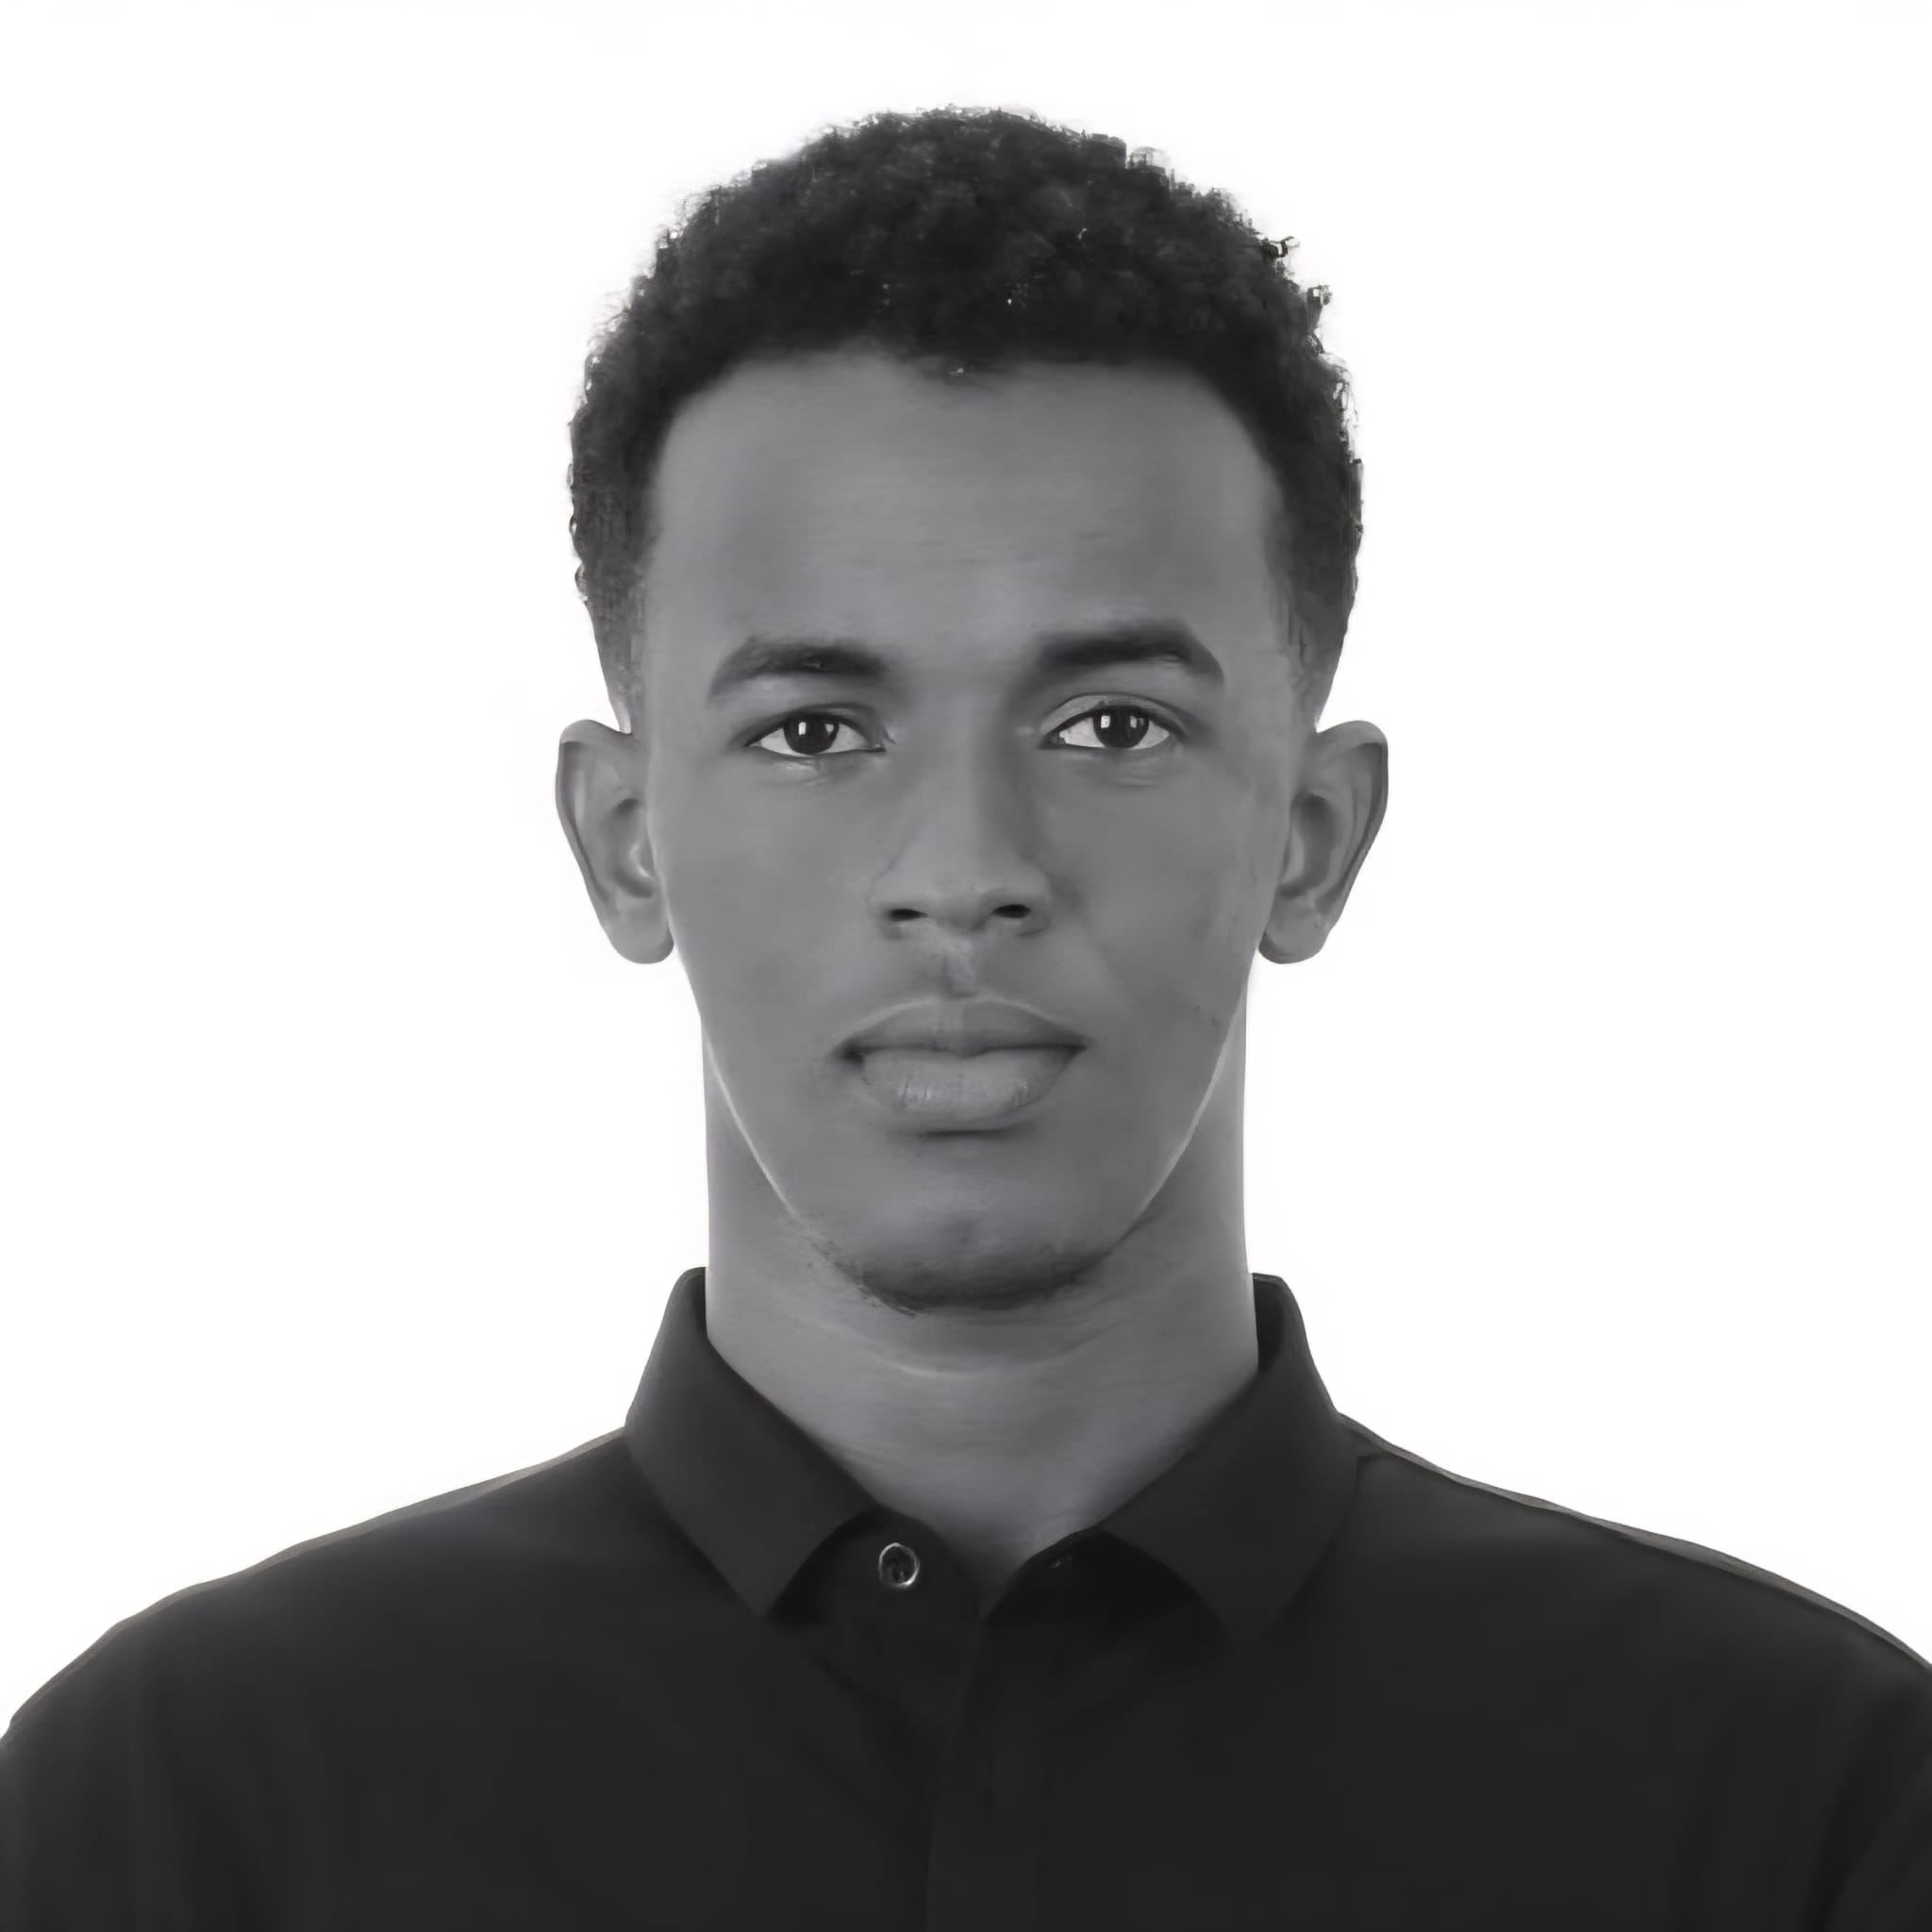
\includegraphics[width=1in,height=1.25in,clip,keepaspectratio]{author_omar.jpeg}}]{Abdirashid Omar}
Abdirashid Omar received the B.Sc. degree in computer science from Bosaso University, Bosaso, Somalia, in 2022. He is currently pursuing the M.Sc. degree with Kookmin University, Seoul, South Korea, and is expected to graduate in August 2026. He is a member of the Vision AI Laboratory, where he conducts research under the supervision of Prof. Jonghyuk Park. His research interests include artificial intelligence, remote sensing, change detection, and computer vision methods.
\end{IEEEbiography}

\begin{IEEEbiography}[{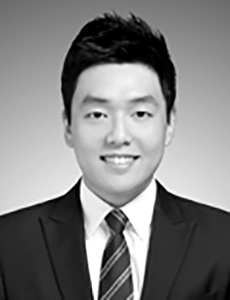
\includegraphics[width=1in,height=1.25in,clip,keepaspectratio]{author_park_bw.png}}]{Jonghyuk Park}
Jonghyuk Park received the B.S. and Ph.D. degrees in industrial engineering from Seoul National University, Seoul, South Korea, in 2015 and 2021, respectively. He worked as a Product Management Engineer at Samsung Electronics in 2015 and was a Research Engineer with ai.m, Seoul, South Korea, from 2020 to 2021. Since 2021, he has been an Assistant Professor with the Department of AI, Big Data and Management, Kookmin University, Seoul, South Korea. His research interests include deep learning, artificial intelligence applications, computer vision, machine learning, and big data analytics.
\end{IEEEbiography}

\end{document}
